\chapter{Biological Background}\label{chap:biointro}

In this chapter, we provide biological background for this work.
We define a genome, describe a DNA sequencing process, and its issues. Then we explain a sequence assembly process, its problems and why it is often not possible to fully assemble the genome.

\section{The Genome}

Each life form is built from at least one cell. One of the most important part of the cell is \emph{DNA (Deoxyribonucleic acid)}, which is located in the cell nucleus (in eukaryotes) or nucleoid (in prokaryotes).
DNA carries the genetic information used for development, functioning and reproduction of the cell or an organism.
DNA is composed of two complementary strands which form a double helix structure. Each strand consists of four types of nucleotides: cytosine (C), guanine (G), adenine (A), or thymine (T).
The nucleotides are arranged in complementary pairs,
i.e.\ if in one strand there is A in the other is T, and if in one is G in the other is C, see Figure~\ref{fig:dnahelix}.
DNA molecules are organized in chromosomes.
The \emph{genome} is a set of all chromosomes in the cell; it includes both the coding and the non-coding parts of DNA.\@
A coding part of the genome is called a gene. Each gene can be translated into a protein sequence which it encodes.

\begin{figure}[htbp]
  \centering
  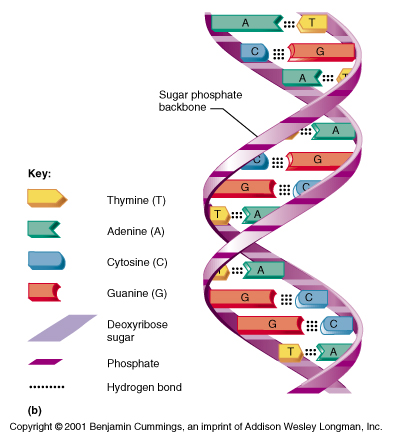
\includegraphics[width=.5\textwidth]{../figures/dna-helix}
  \caption[DNA double helix]{The DNA double helix. Each strand consists of many nucleotides. The nucleotides A---T, and C---G are complementary~\cite{dnahelix}.}\label{fig:dnahelix}
\end{figure}

Parts of the DNA sequence may be repeated many times in the genome. These parts are called repeats. Also genes may occur multiple times in the genome. Such group of similar genes is called a gene family (see Chapter~\ref{chap:repeatsfamilies}).

\section{DNA Sequencing}

Obtaining a DNA sequence or its part from a cell is called \emph{DNA sequencing}.
DNA sequencing includes experimental methods of extracting the DNA sequence from the cell and the computational analysis of sequencing data called sequence assembly.

The first sequenced genome was a simple RNA virus in 1976. The 3.2Gb long human genome was first sequenced in 2001, and it took 13 years and cost about 3 billions dollars~\cite{venter2001sequence}. Nowadays it is possible to sequence such a large genome at a much lower cost (several tens thousands dollars).

The traditional sequencing method, called \emph{Sanger sequencing}, was developed by Frederick Sanger in 1977~\cite{sanger1977dna}. It was used in the first human genome sequencing.
In the Sanger sequencing, a double stranded DNA is first split into the single strand DNA.\@ The single strand DNA can be used as a template to create its copies, if particular enzymes and sufficient amount of nucleotides is available. The key role in Sanger sequencing is played by modified nucleotides. The nucleotides are modified in two ways: they are colored by a florescent coloring and modified, so the DNA copy process cannot continue after the nucleotide. This results in DNA segments of various lengths, which are the prefixes of the sequenced DNA interrupted by the colored nucleotide in their last position. Each length is represented by multiple segments. The segments are then ordered by length using electrophoresis, and the colors are read from the shortest to the longest segment, forming a DNA sequence (Figure~\ref{fig:sanger}).

\begin{figure}[htbp]
  \centering
  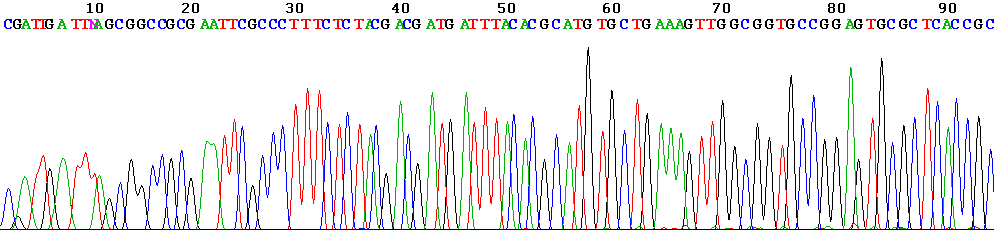
\includegraphics[width=\textwidth]{../figures/sanger}
  \caption[Sanger sequencing]{Example of a Sanger sequencing read. The four bases are detected using different fluorescent labels. These are detected and represented as `peaks' of different colors, which can then be interpreted to determine the base sequence, shown at the top~\cite{wiki:sanger-img}.}\label{fig:sanger}
\end{figure}

Only short sequences, up to 500--1000 bases, can be read in this way. Therefore the original DNA has to be split into many overlapping short sequences.
Therefore instead of one long sequence per chromosome, we get many short sequences, called reads, which have to be assembled together to obtain the original sequence.

Since 2005, sequencing machines of the second generation (or the new generation sequencing machines) have been commercially available. There are multiple different technologies for \emph{new generation sequencing (NGS)}, but they all share some properties.
They produce a huge amount of reads from the same sample, and are faster and cheaper. They also produce much shorter reads (35--400 bases) than the Sanger sequencing, which makes a DNA assembly even harder task.

%todo{pacbio ma dlhsie ready, ale je to este NGS?, da sa mozno blizsie popisat ready z illuminy, uvidime ako vyjde cas}

\section{Sequence Assembly}
\label{sect:dna-assembly}

The sequence assembly aims to reconstruct a whole DNA sequence from short sequencing reads. Ideally, we would get a single sequence per chromosome. In reality, there are usually several problems causing the final sequence to be split into multiple contigs.

The first aspect, which can influence the final sequence assembly quality is the coverage of input data. The coverage is the average number of reads covering a single base in the genome (see Chapter~\ref{chap:genomesize} for more details).
As the bases are not covered uniformly, some of the bases may not be covered at all. Those bases are then missing from the assembly and causing the final sequence to be cut at that place. With increasing coverage, the probability that a base would not be covered decreases.
Moreover, the reads may contain errors and the final sequence is built as the consensus sequence, in which each base is computed as the consensus from all reads overlapping the base. If a base is covered with very few reads it may happen, that the consensus will be wrong. Again, with increasing coverage, the probability that this happens decreases. Thus, the higher the coverage, the better the quality of the sequence.

The other problem of the sequence assembly is caused by repetitive sequences. These sequences are often longer than the read length. Thus, there may be several reads from different copies of the repetitive sequence, which may look very similar, and are hard to distinguish. If such repeats occur in tandem, it is then very hard to find out the correct length of the repetitive region. If the repeats occur randomly in the genome, it may be hard to find out the order of the parts of genome which lay between the repeat occurrences.

There are two main approaches used in modern genome assemblers. The first is based on overlap-layout-consensus framework (e.g.\ Celera~\cite{myers2000celera}, SGA~\cite{simpson2010sga}). The second is based on de Bruin graphs~\cite{deBruijn} (e.g.\ Velvet~\cite{zerbino2008velvet}, ALLPATHS-LG~\cite{gnerre2011allpaths}). Both this methods construct a string graph~\cite{myers2005stringgraph} from the sequencing data, but they differ in the process of its creation.

The vertices in a string graph are all unambiguous sequences, and the edges are between those which are overlapping. An Euler tour in a string graph forms a possible assembly. (Figure~\ref{fig:string-graph})

\begin{figure}[htbp]
  \centering
  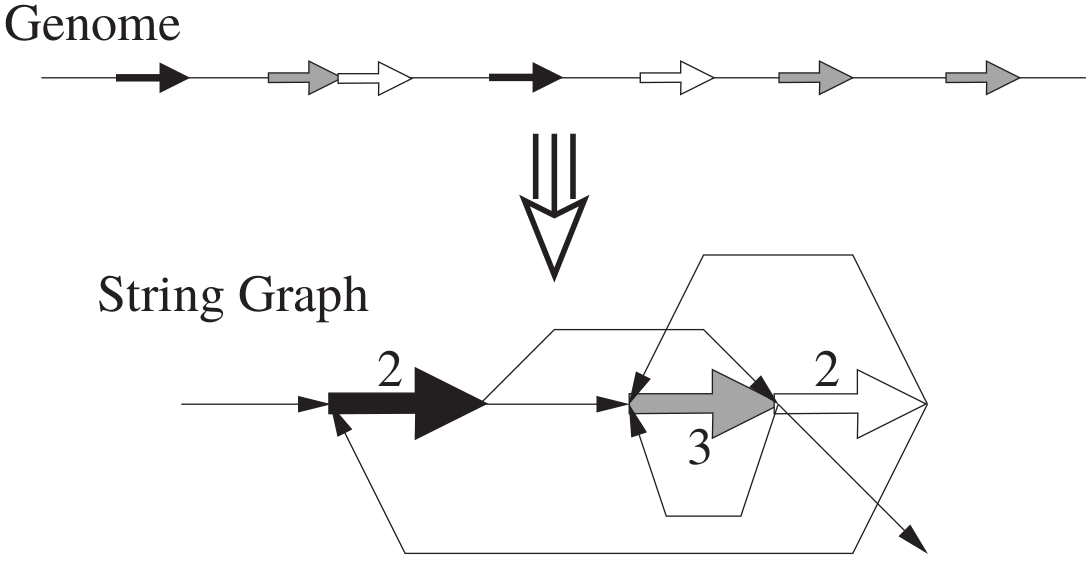
\includegraphics[width=0.5\textwidth]{../figures/string-graph.png}
  \caption[String graph]{A string graph constructed from a genome.
  Each shaded arrow represents a copy of repetitive sequence.
  The like repetitive sequences are collapsed together in the string graph~\cite{myers2005stringgraph}.}\label{fig:string-graph}
\end{figure}

To resolve a repetitive sequence lengths and order of the parts of genome, some assemblers  (e.g.\ ALLPATHS-LG~\cite{gnerre2011allpaths}) use paired reads, which can be obtained from the NGS machines, as additional data. The paired reads are pairs of reads, for which we know approximate distance in the genome. Multiple distance paired reads can be combined together, to get better result.
